\chapter{METHODOLOGY}
\label{ch:methodology}

\section{Methodological Approach}

This thesis follows a system design-and-implementation methodology focused on backend engineering. The method combines requirement analysis, architecture design, workflow modeling, and evaluation planning before detailed implementation.

The objective of this chapter is to define how the backend is designed to satisfy practical requirements for security, consistency, scalability, and real-time support continuity.

\subsection{Design Process}

The design process is executed in five stages:
\begin{itemize}
    \item Stage 1: derive requirements from target user flows (account, cart, checkout, payment, support).
    \item Stage 2: define module boundaries for API, business logic, and persistence.
    \item Stage 3: model data and transaction-critical workflows.
    \item Stage 4: model real-time support workflows with escalation and reassignment.
    \item Stage 5: define evaluation criteria for performance and reliability.
\end{itemize}

\section{Backend Requirement Specification}

\subsection{Functional Requirements}

\begin{table}[H]
\centering
\caption{Core Functional Requirements}
\label{tab:method-functional-requirements}
\begin{tabular}{|p{1.2cm}|p{5.6cm}|p{5.2cm}|}
\hline
\textbf{ID} & \textbf{Requirement} & \textbf{Design Intent} \\
\hline
FR1 & Authentication and session lifecycle management & Secure login state, token rotation, and session revocation \\
\hline
FR2 & Product catalog and filtering APIs & Fast product discovery with stock-aware payloads \\
\hline
FR3 & Cart lifecycle operations & Correct add/update/remove behavior with stock validation \\
\hline
FR4 & Checkout reservation control & Atomic reservation for stock and voucher quotas \\
\hline
FR5 & Payment callback finalization & Verified callback processing and idempotent order updates \\
\hline
FR6 & Real-time AI chat with human handoff & Continuous support flow with staff assignment and fallback \\
\hline
\end{tabular}
\end{table}

\subsection{Non-Functional Requirements}

\begin{table}[H]
\centering
\caption{Non-Functional Requirements and Targets}
\label{tab:method-nonfunctional-requirements}
\begin{tabular}{|p{2.8cm}|p{3.8cm}|p{5.4cm}|}
\hline
\textbf{Category} & \textbf{Target} & \textbf{Design Strategy} \\
\hline
Performance & Stable API latency under concurrent load & Redis-assisted coordination and optimized service boundaries \\
\hline
Consistency & No over-reservation of stock and vouchers & Atomic Redis/Lua reservation and TTL-based rollback \\
\hline
Security & Protected access and trusted callbacks & JWT validation, session control, signature verification \\
\hline
Reliability & Safe recovery from partial failures & Idempotent payment handling and explicit error boundaries \\
\hline
Maintainability & Clear module ownership & Route-controller-service-repository layering \\
\hline
\end{tabular}
\end{table}

\section{System Design}

\subsection{Overall Backend Architecture}

The backend uses a modular monolithic architecture with Express for HTTP APIs and Socket.IO for realtime channels. PostgreSQL is the transactional source of truth, while Redis is used for short-lived coordination state such as reservation counters, chat session metadata, and heartbeat TTL keys.

\begin{figure}[H]
\centering
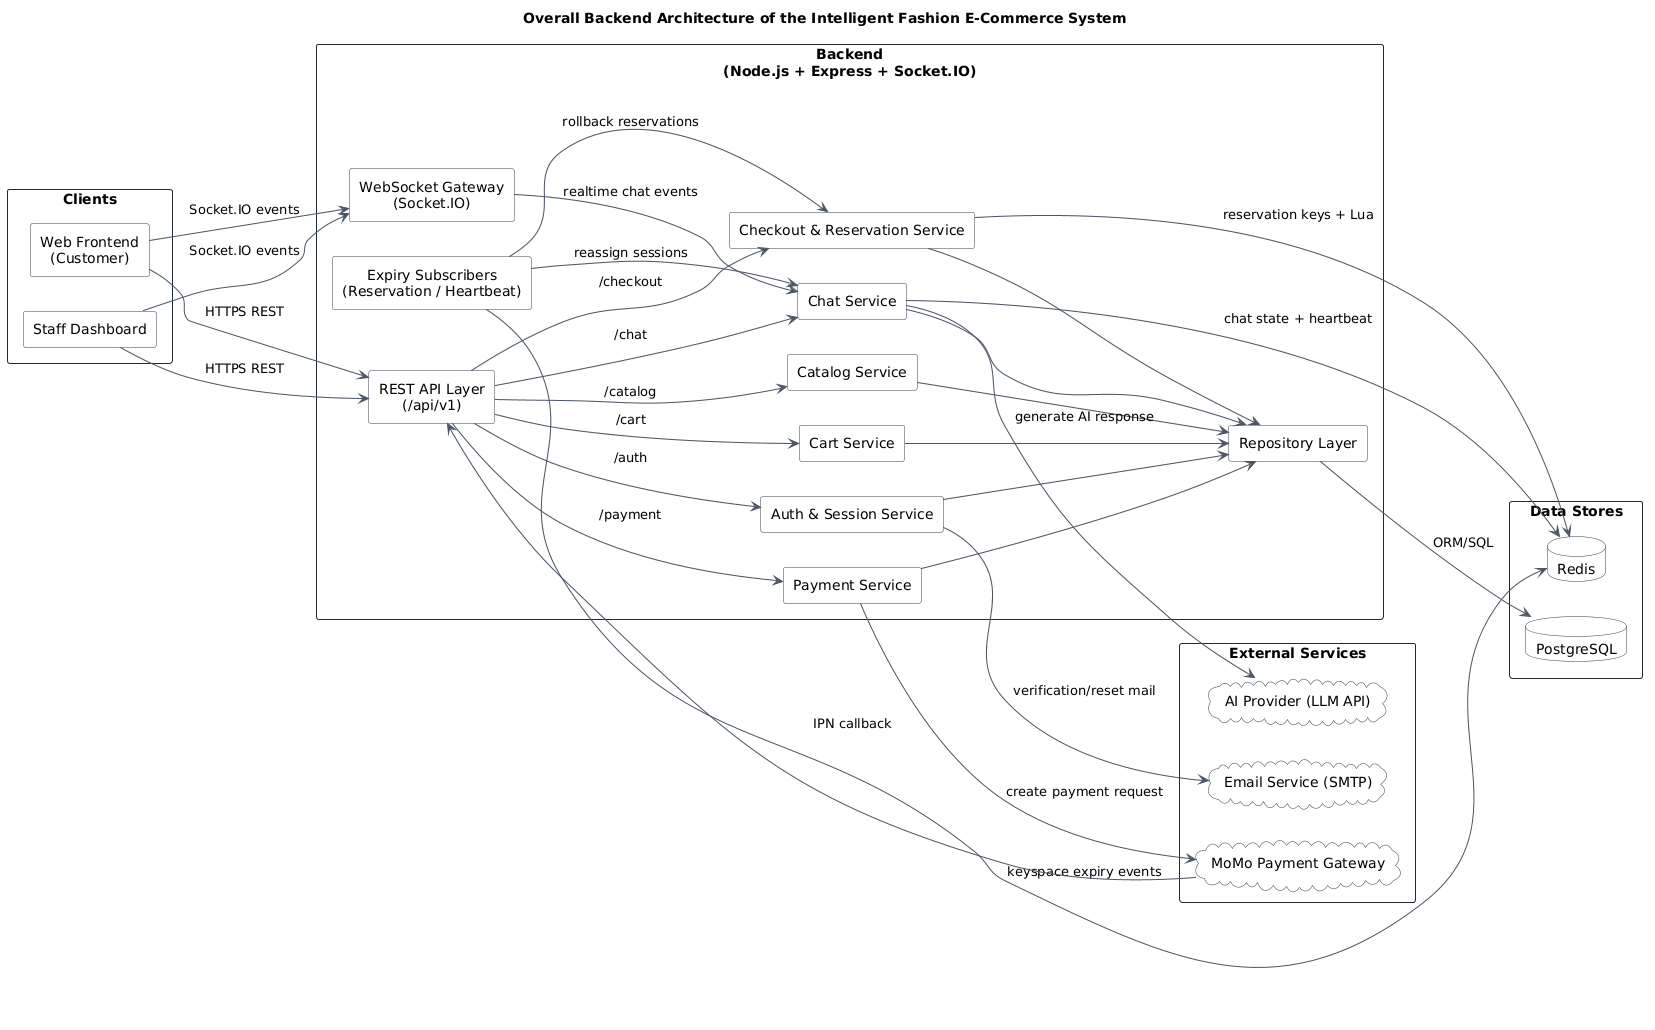
\includegraphics[width=0.9\textwidth]{figures/ch3_system_architecture.png}
\caption{Overall Backend Architecture}
\label{fig:method-backend-architecture}
\end{figure}

\subsection{Data Design and Entity Relationships}

The persistence model captures account, catalog, cart, order, discount, and chat domains. Entity relationships are designed to support both transactional operations (checkout and payment) and conversational support workflows (sessions, messages, transfers).

\begin{figure}[H]
\centering
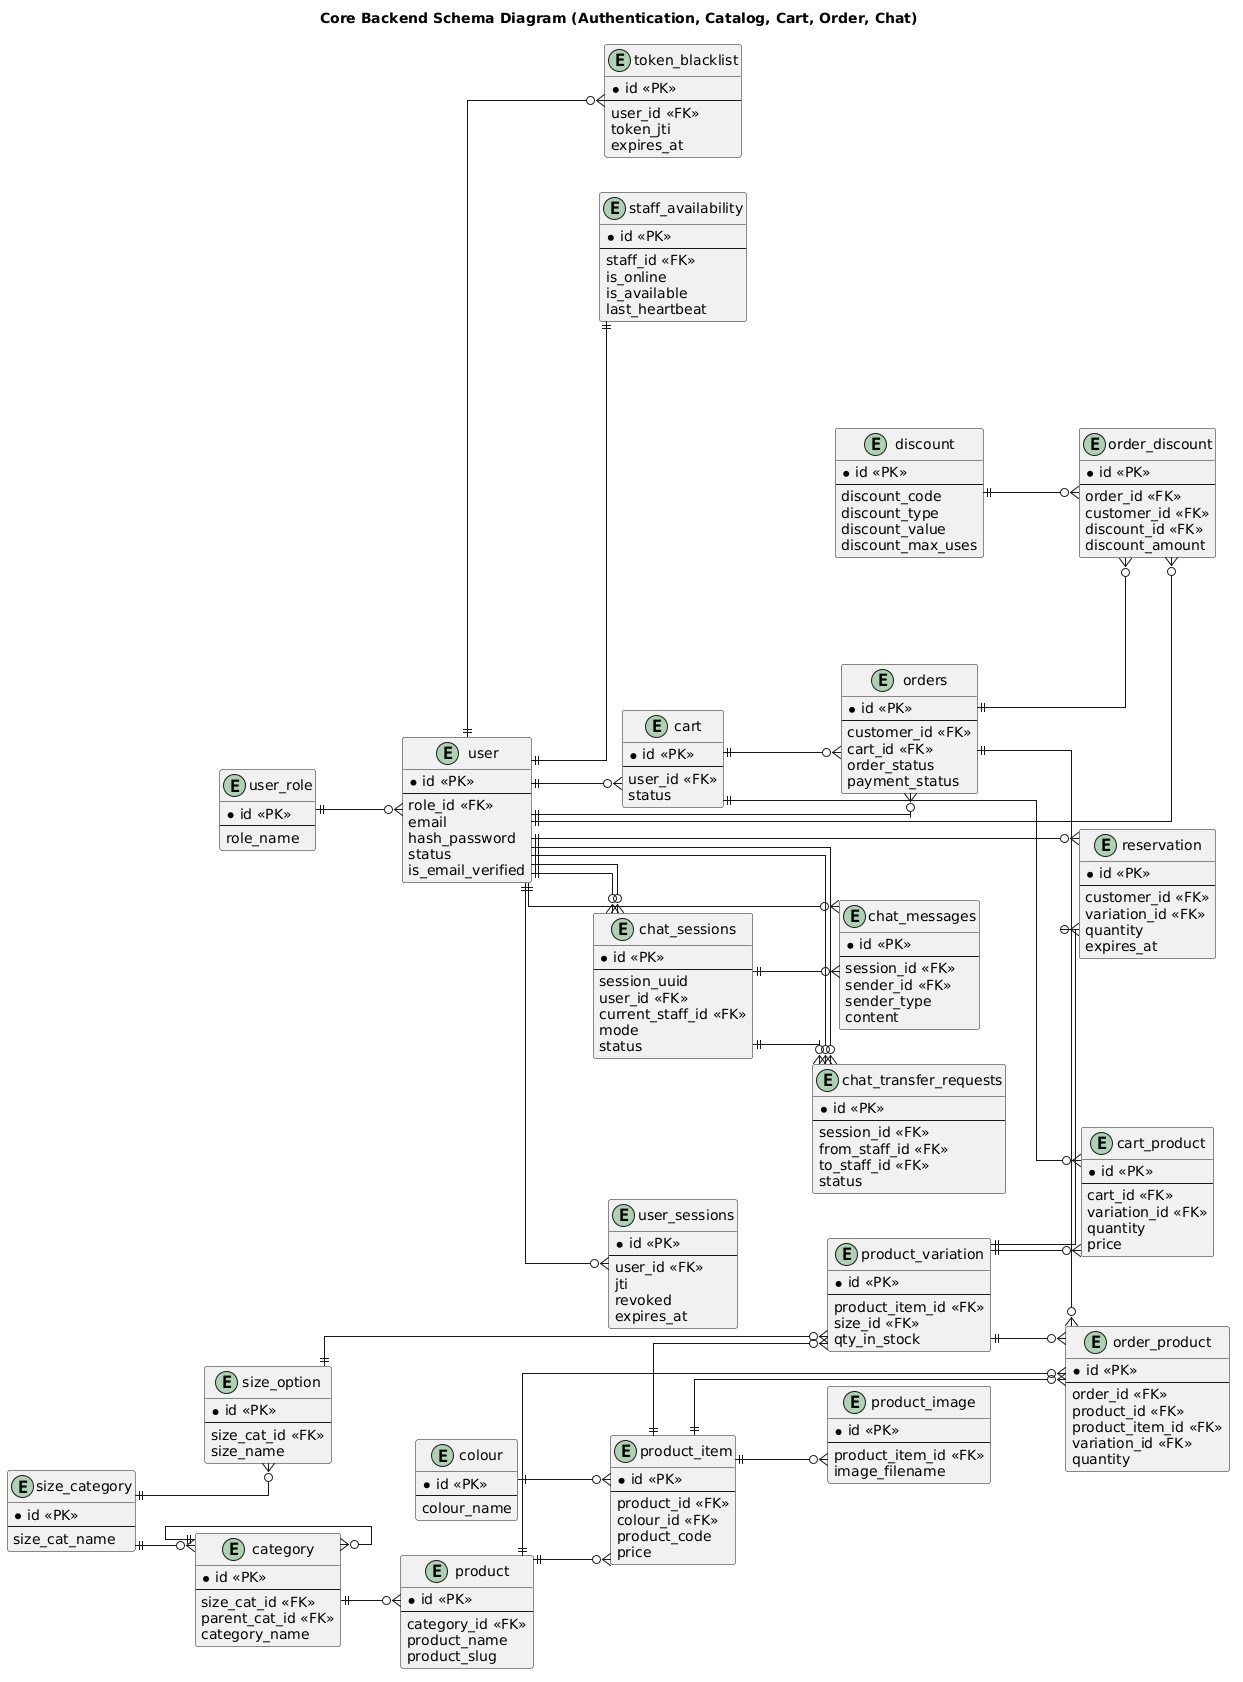
\includegraphics[width=0.9\textwidth]{figures/ch3_backend_schema.png}
\caption{Core Backend Schema Diagram}
\label{fig:method-backend-erd}
\end{figure}

\subsection{Use Case Boundary}

Use case modeling is used to define external actor interactions with the backend, including customer actions, support staff operations, and payment provider callbacks.

\begin{figure}[H]
\centering
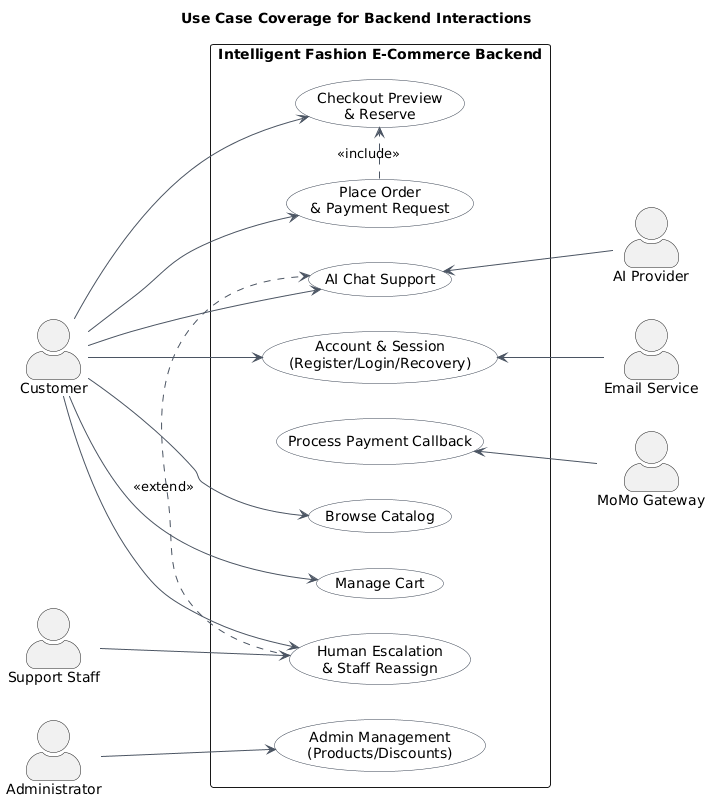
\includegraphics[width=\textwidth,height=0.78\textheight,keepaspectratio]{figures/ch3_use_case.png}
\caption{Use Case Coverage for Backend Interactions}
\label{fig:method-backend-usecase}
\end{figure}

\section{Workflow Modeling for Core Features}

\subsection{Authentication and Account Recovery Workflow}

This workflow includes registration, email verification, login, refresh token, logout, and password recovery. The model emphasizes token lifecycle control and secure account restoration.

\begin{figure}[H]
\centering
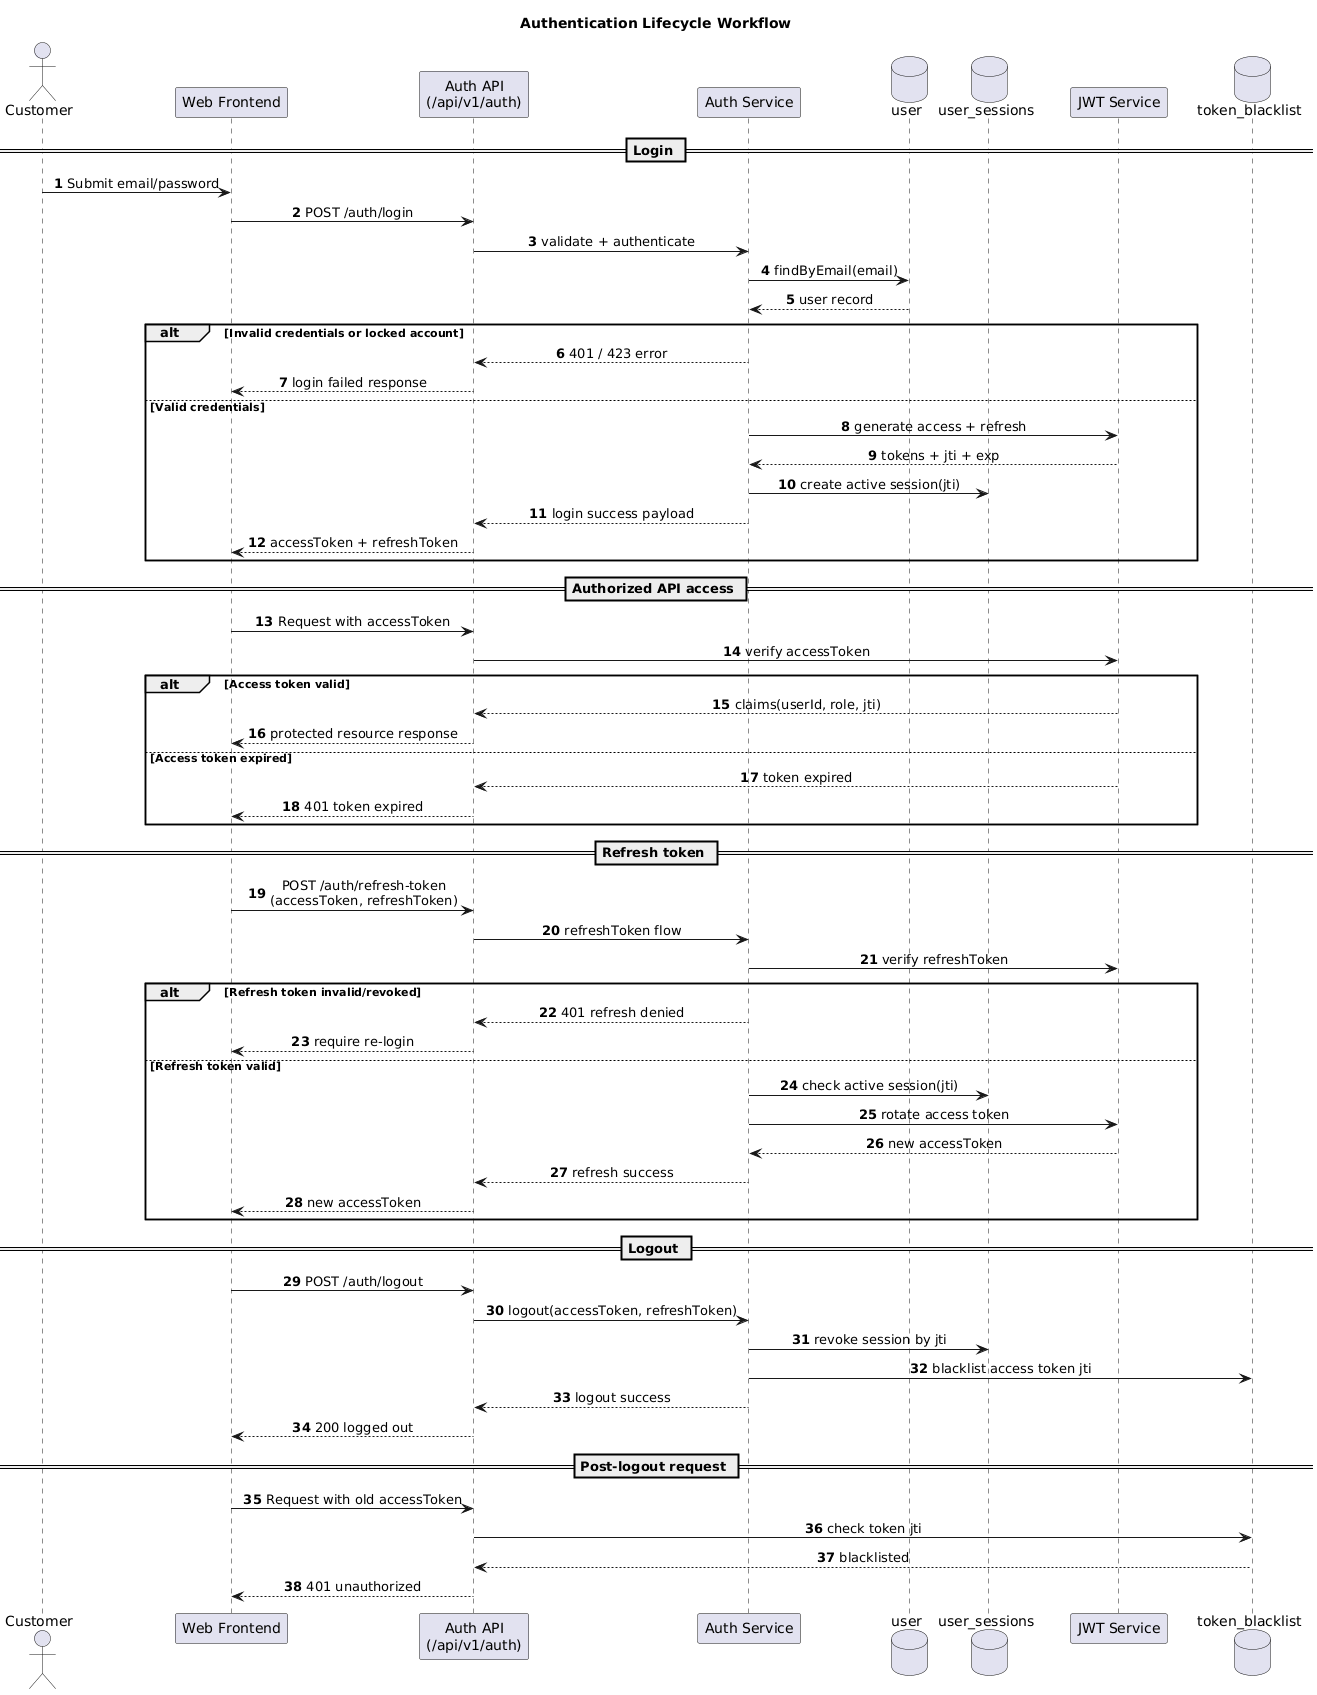
\includegraphics[width=0.9\textwidth]{figures/ch3_auth_lifecycle.png}
\caption{Authentication Lifecycle Workflow}
\label{fig:method-auth-lifecycle}
\end{figure}

\begin{figure}[H]
\centering
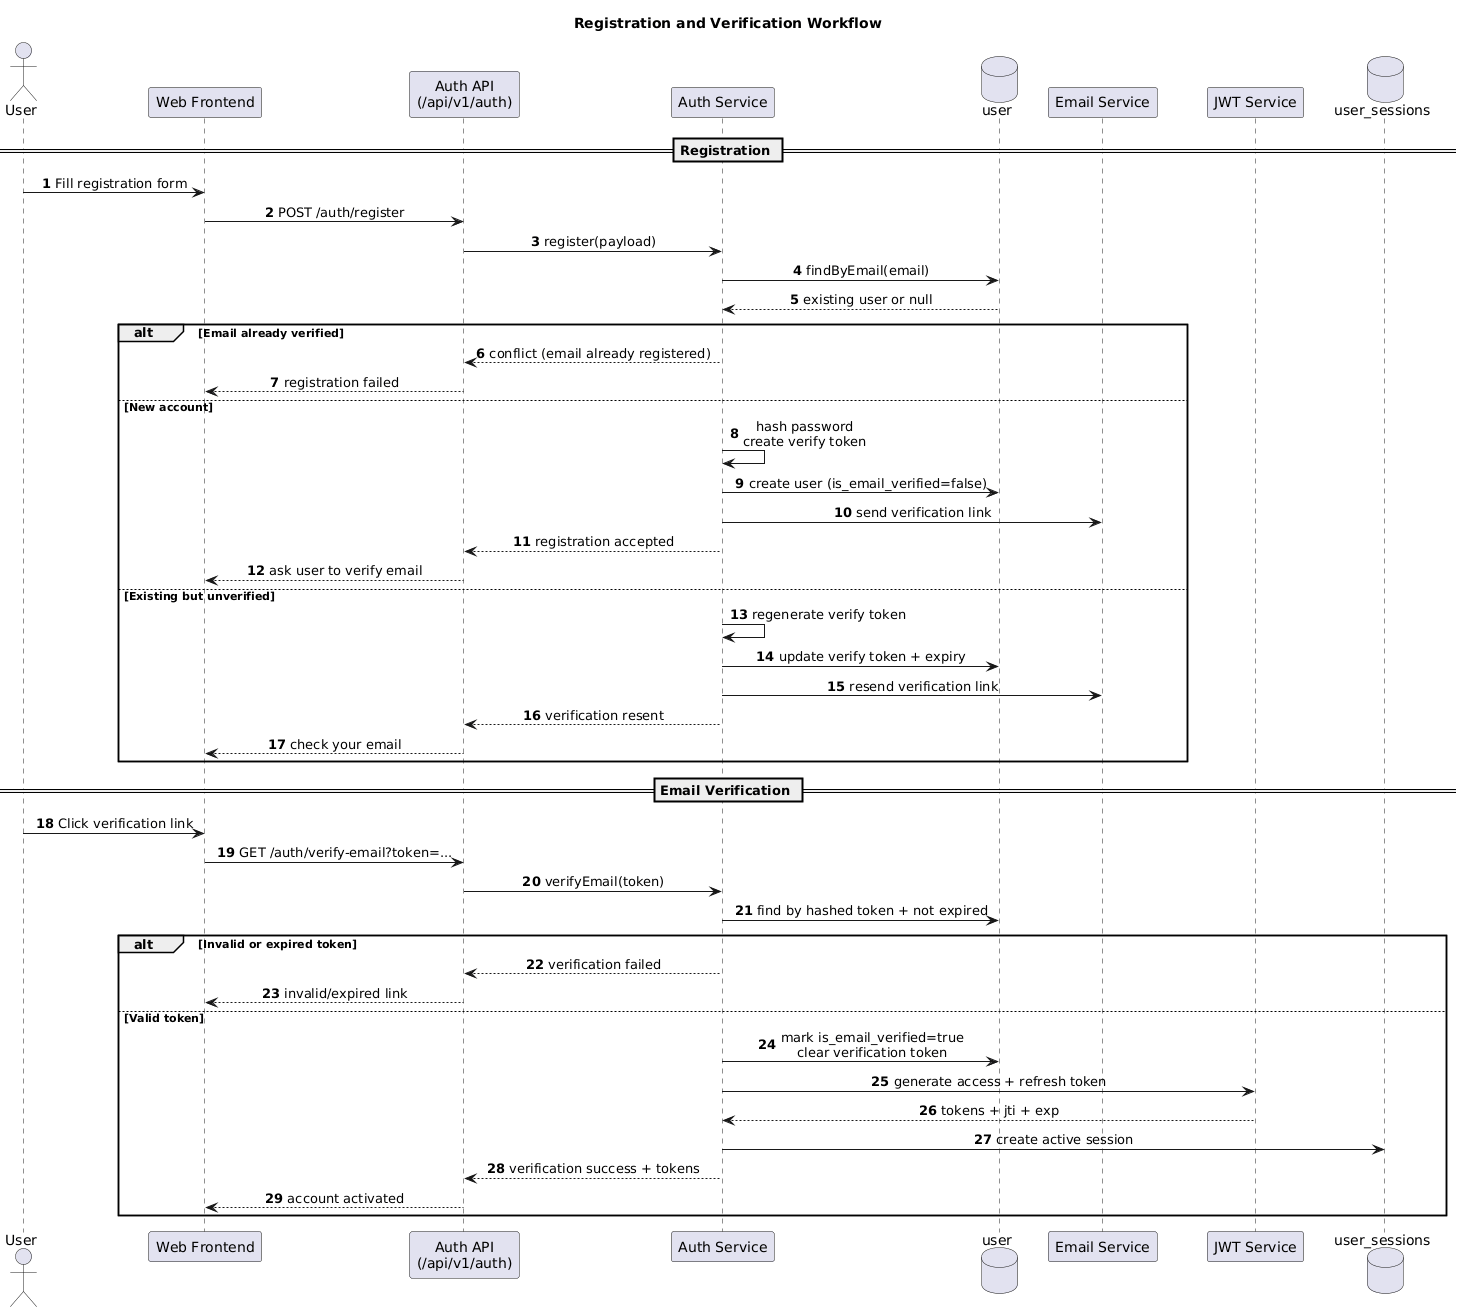
\includegraphics[width=0.9\textwidth]{figures/ch3_registration_verification.png}
\caption{Registration and Verification Workflow}
\label{fig:method-registration-workflow}
\end{figure}

\begin{figure}[H]
\centering
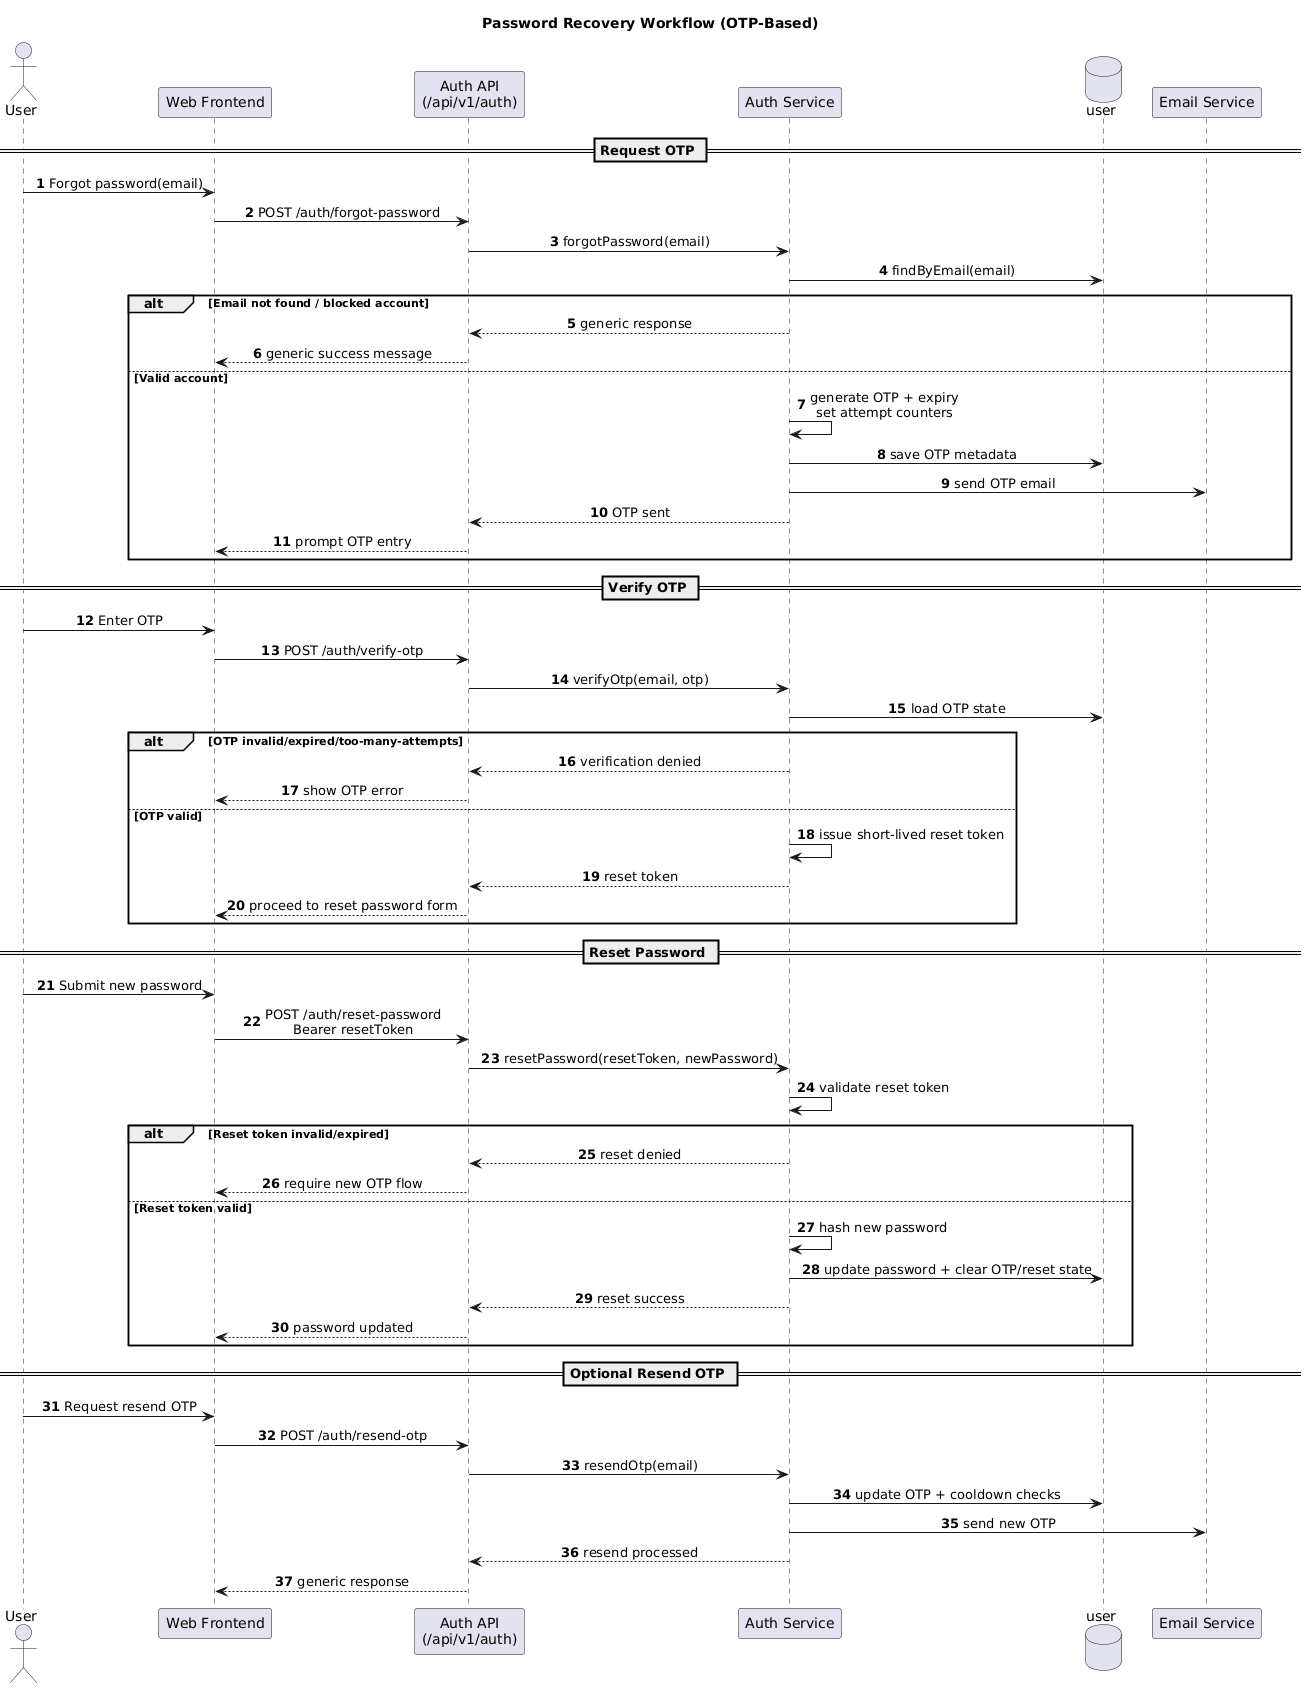
\includegraphics[width=0.9\textwidth]{figures/ch3_password_recovery.png}
\caption{Password Recovery Workflow}
\label{fig:method-recovery-workflow}
\end{figure}

\subsection{Catalog, Cart, and Checkout Workflow}

This workflow models product selection, cart mutation, checkout preview, and reservation setup. It focuses on preventing race conditions during high-concurrency purchase attempts.

\begin{figure}[H]
\centering
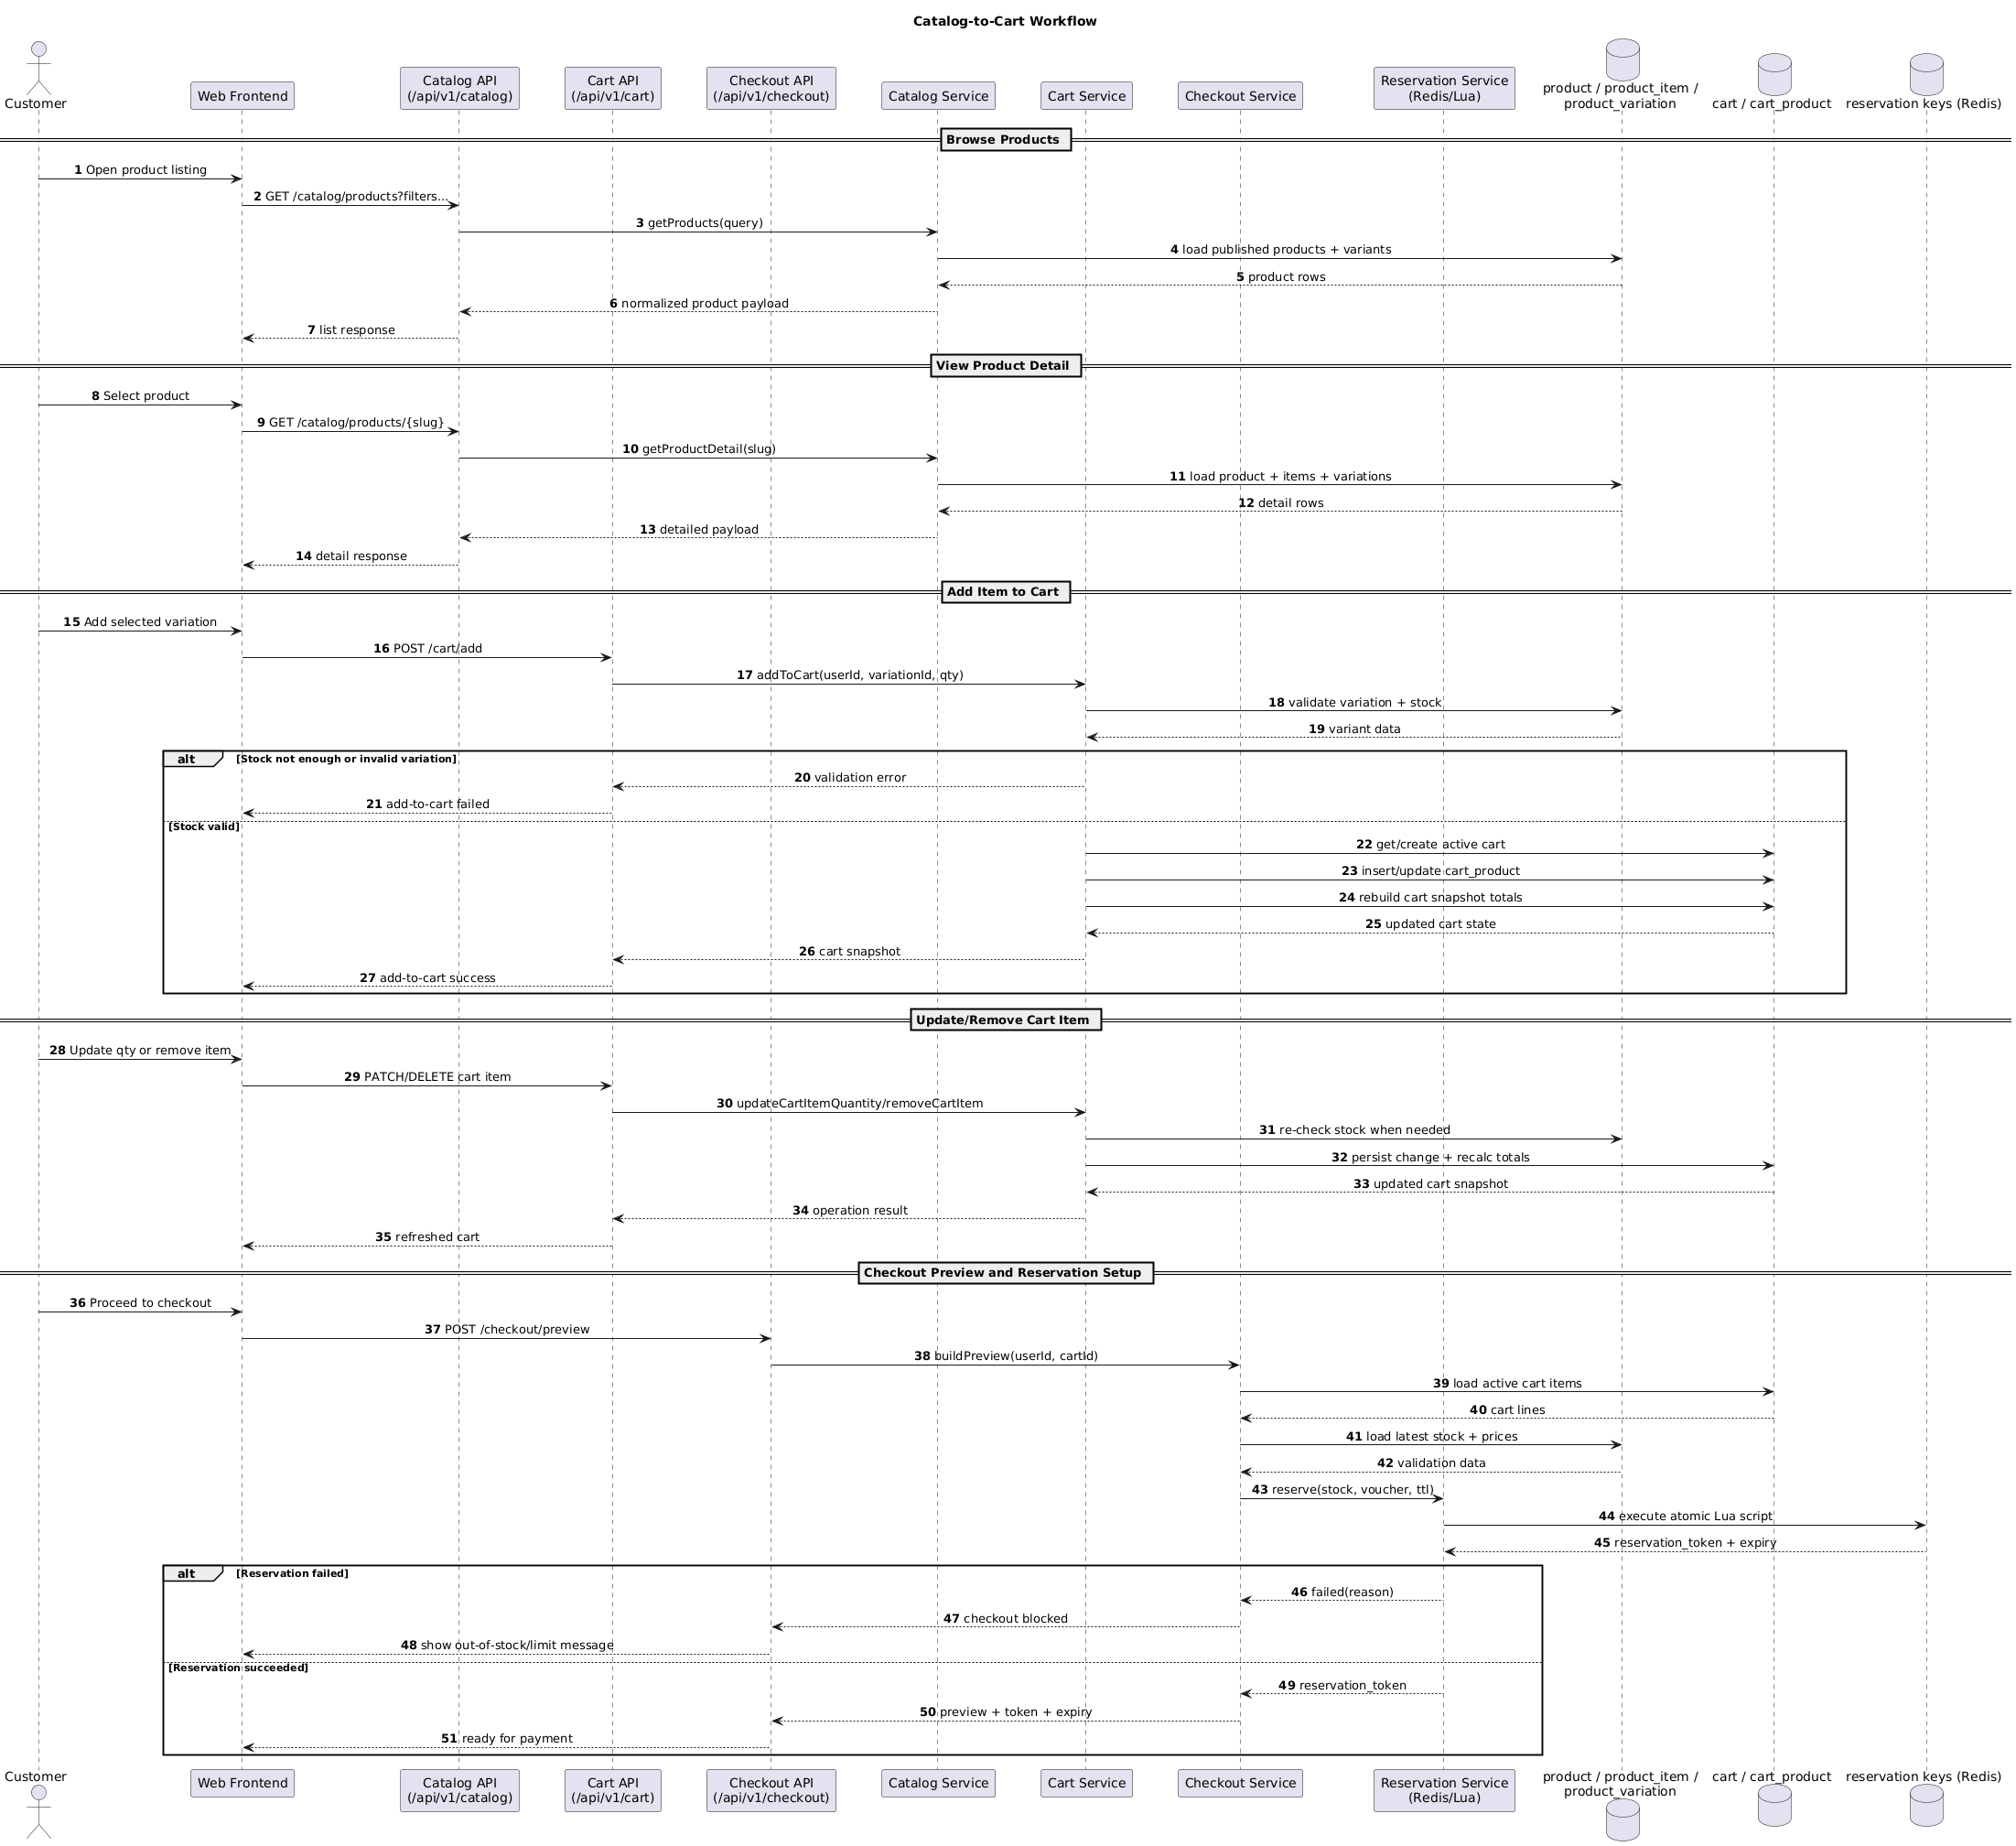
\includegraphics[width=0.9\textwidth]{figures/ch3_catalog_cart_flow.png}
\caption{Catalog-to-Cart Workflow}
\label{fig:method-catalog-cart-workflow}
\end{figure}

\subsection{Payment Finalization Workflow}

This workflow captures callback verification, order-state reconciliation, and idempotent finalization.

\begin{figure}[H]
\centering
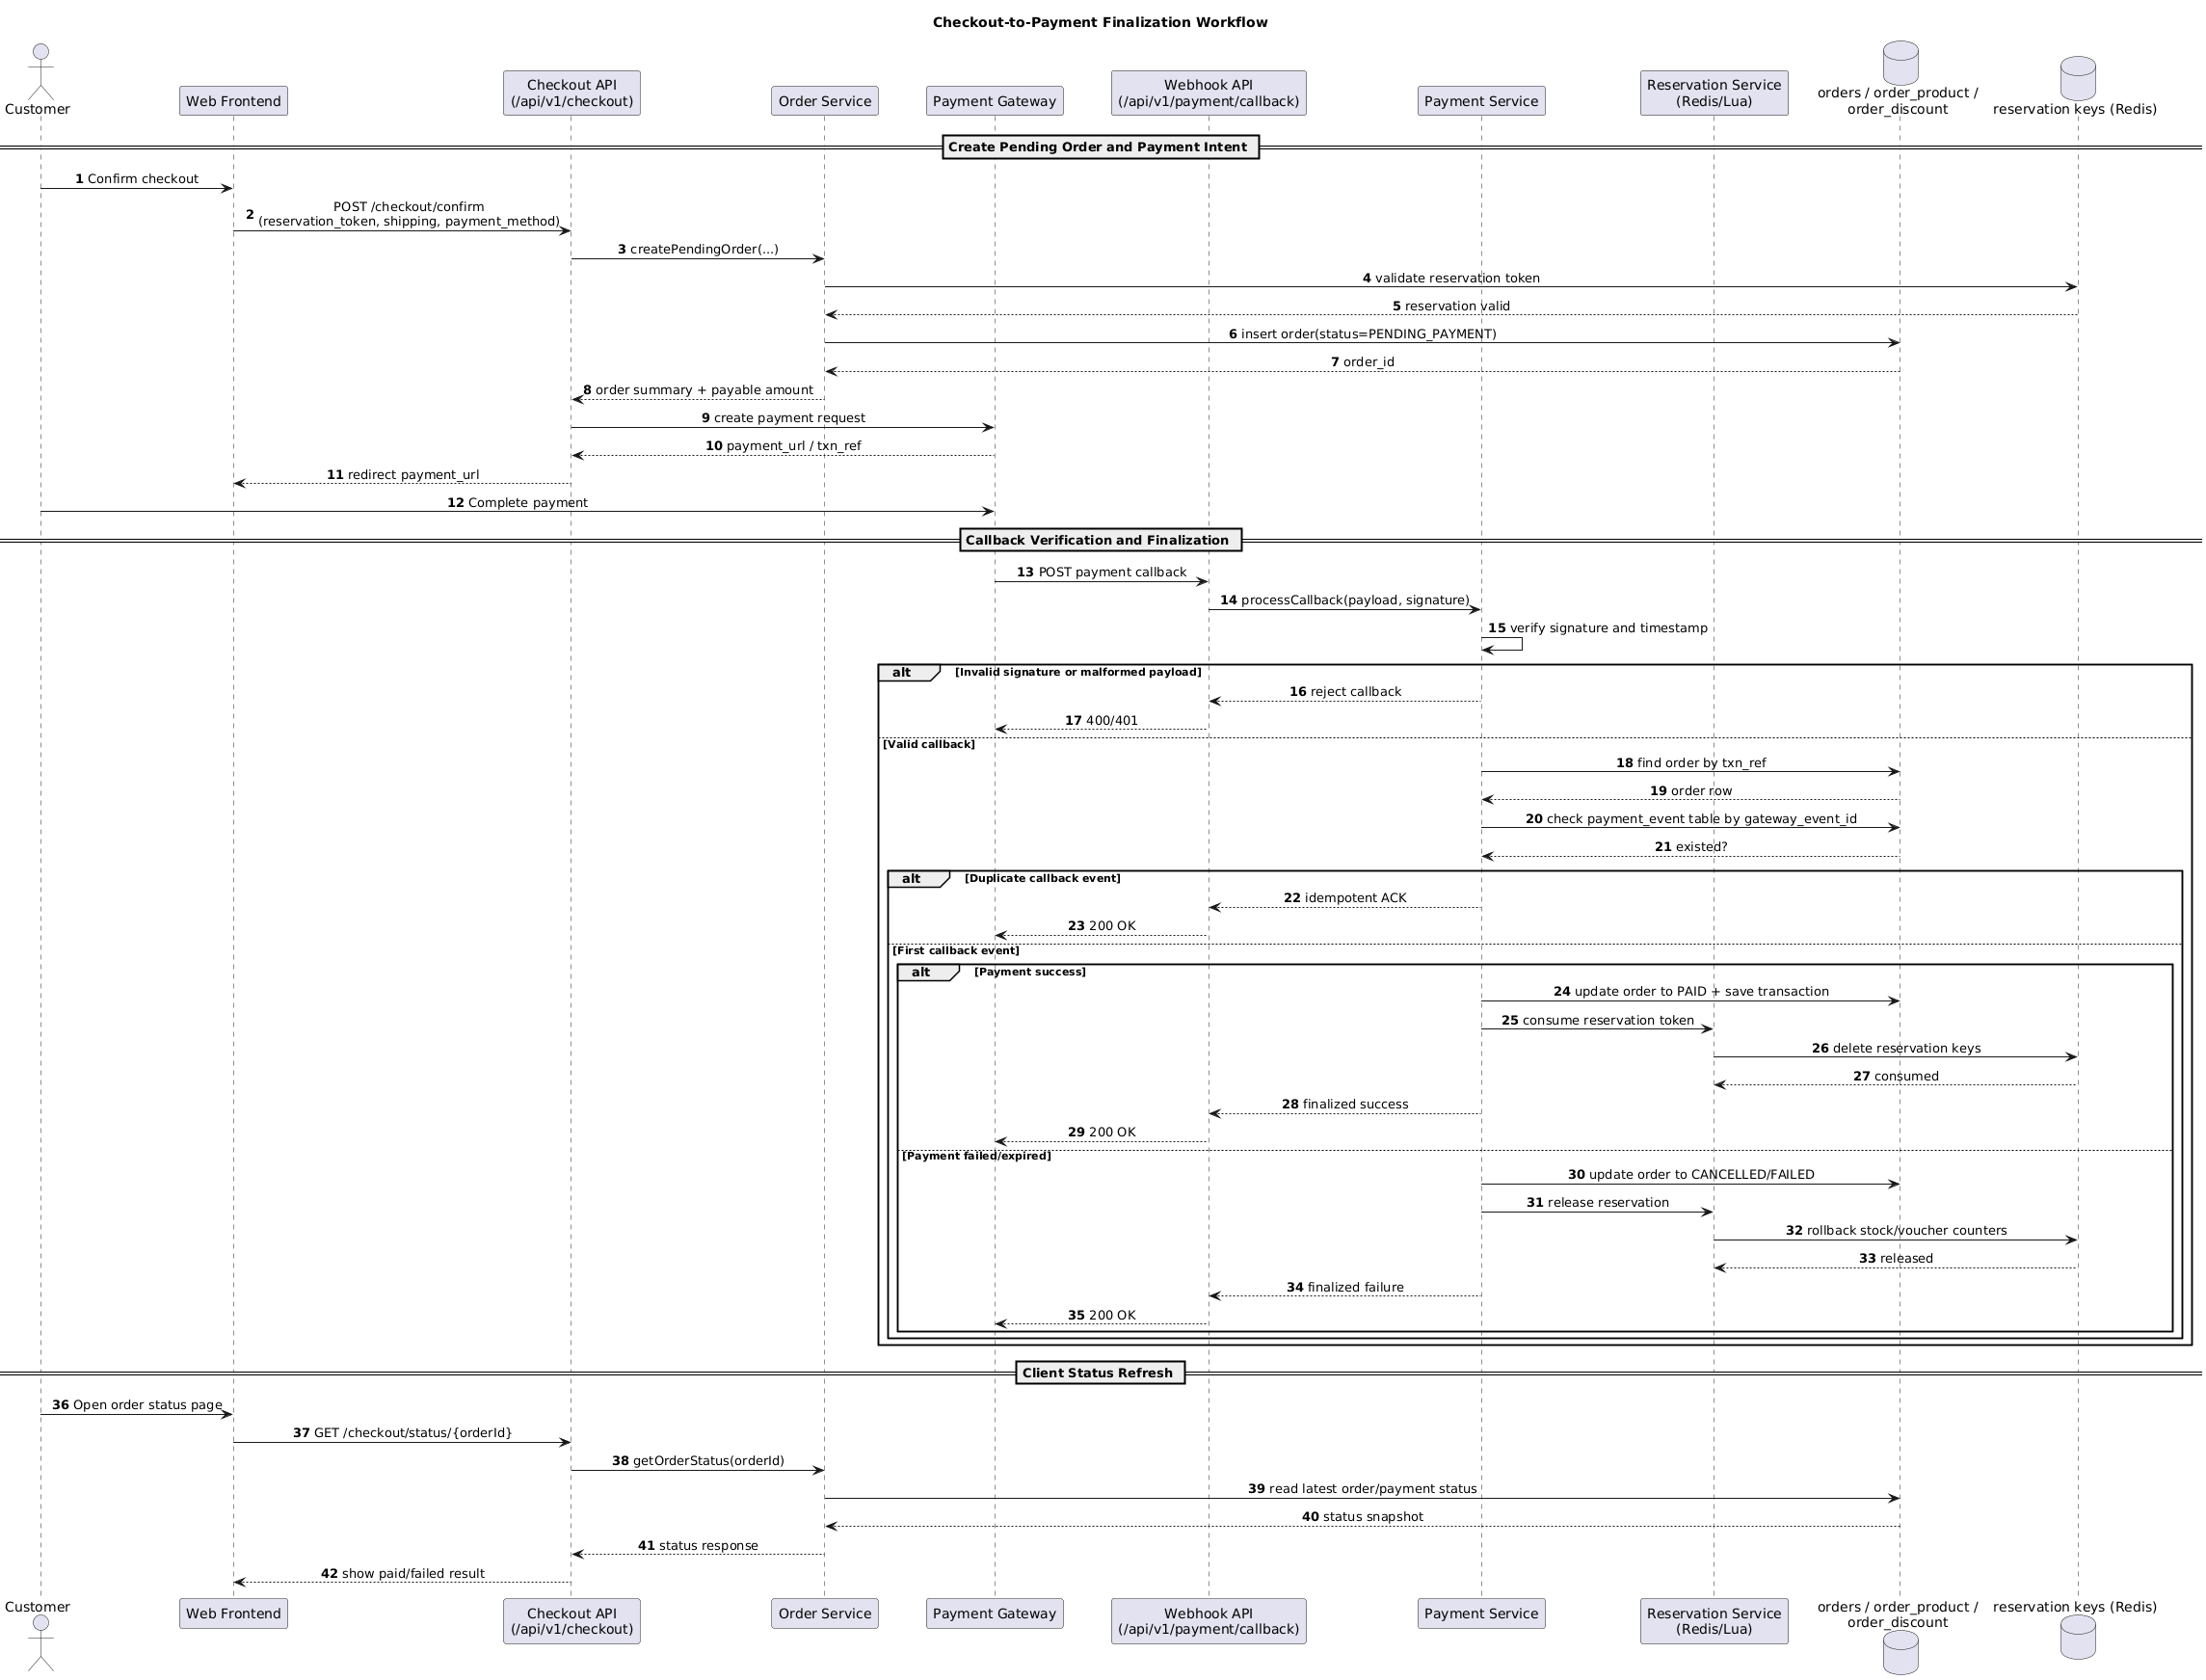
\includegraphics[width=0.9\textwidth]{figures/ch3_payment_finalization_flow.png}
\caption{Checkout-to-Payment Finalization Workflow}
\label{fig:method-payment-workflow}
\end{figure}

\subsection{AI Chat and Human Handoff Workflow}

This workflow models realtime conversation handling, escalation to staff, and continuity mechanisms when staff availability changes.

\begin{figure}[H]
\centering
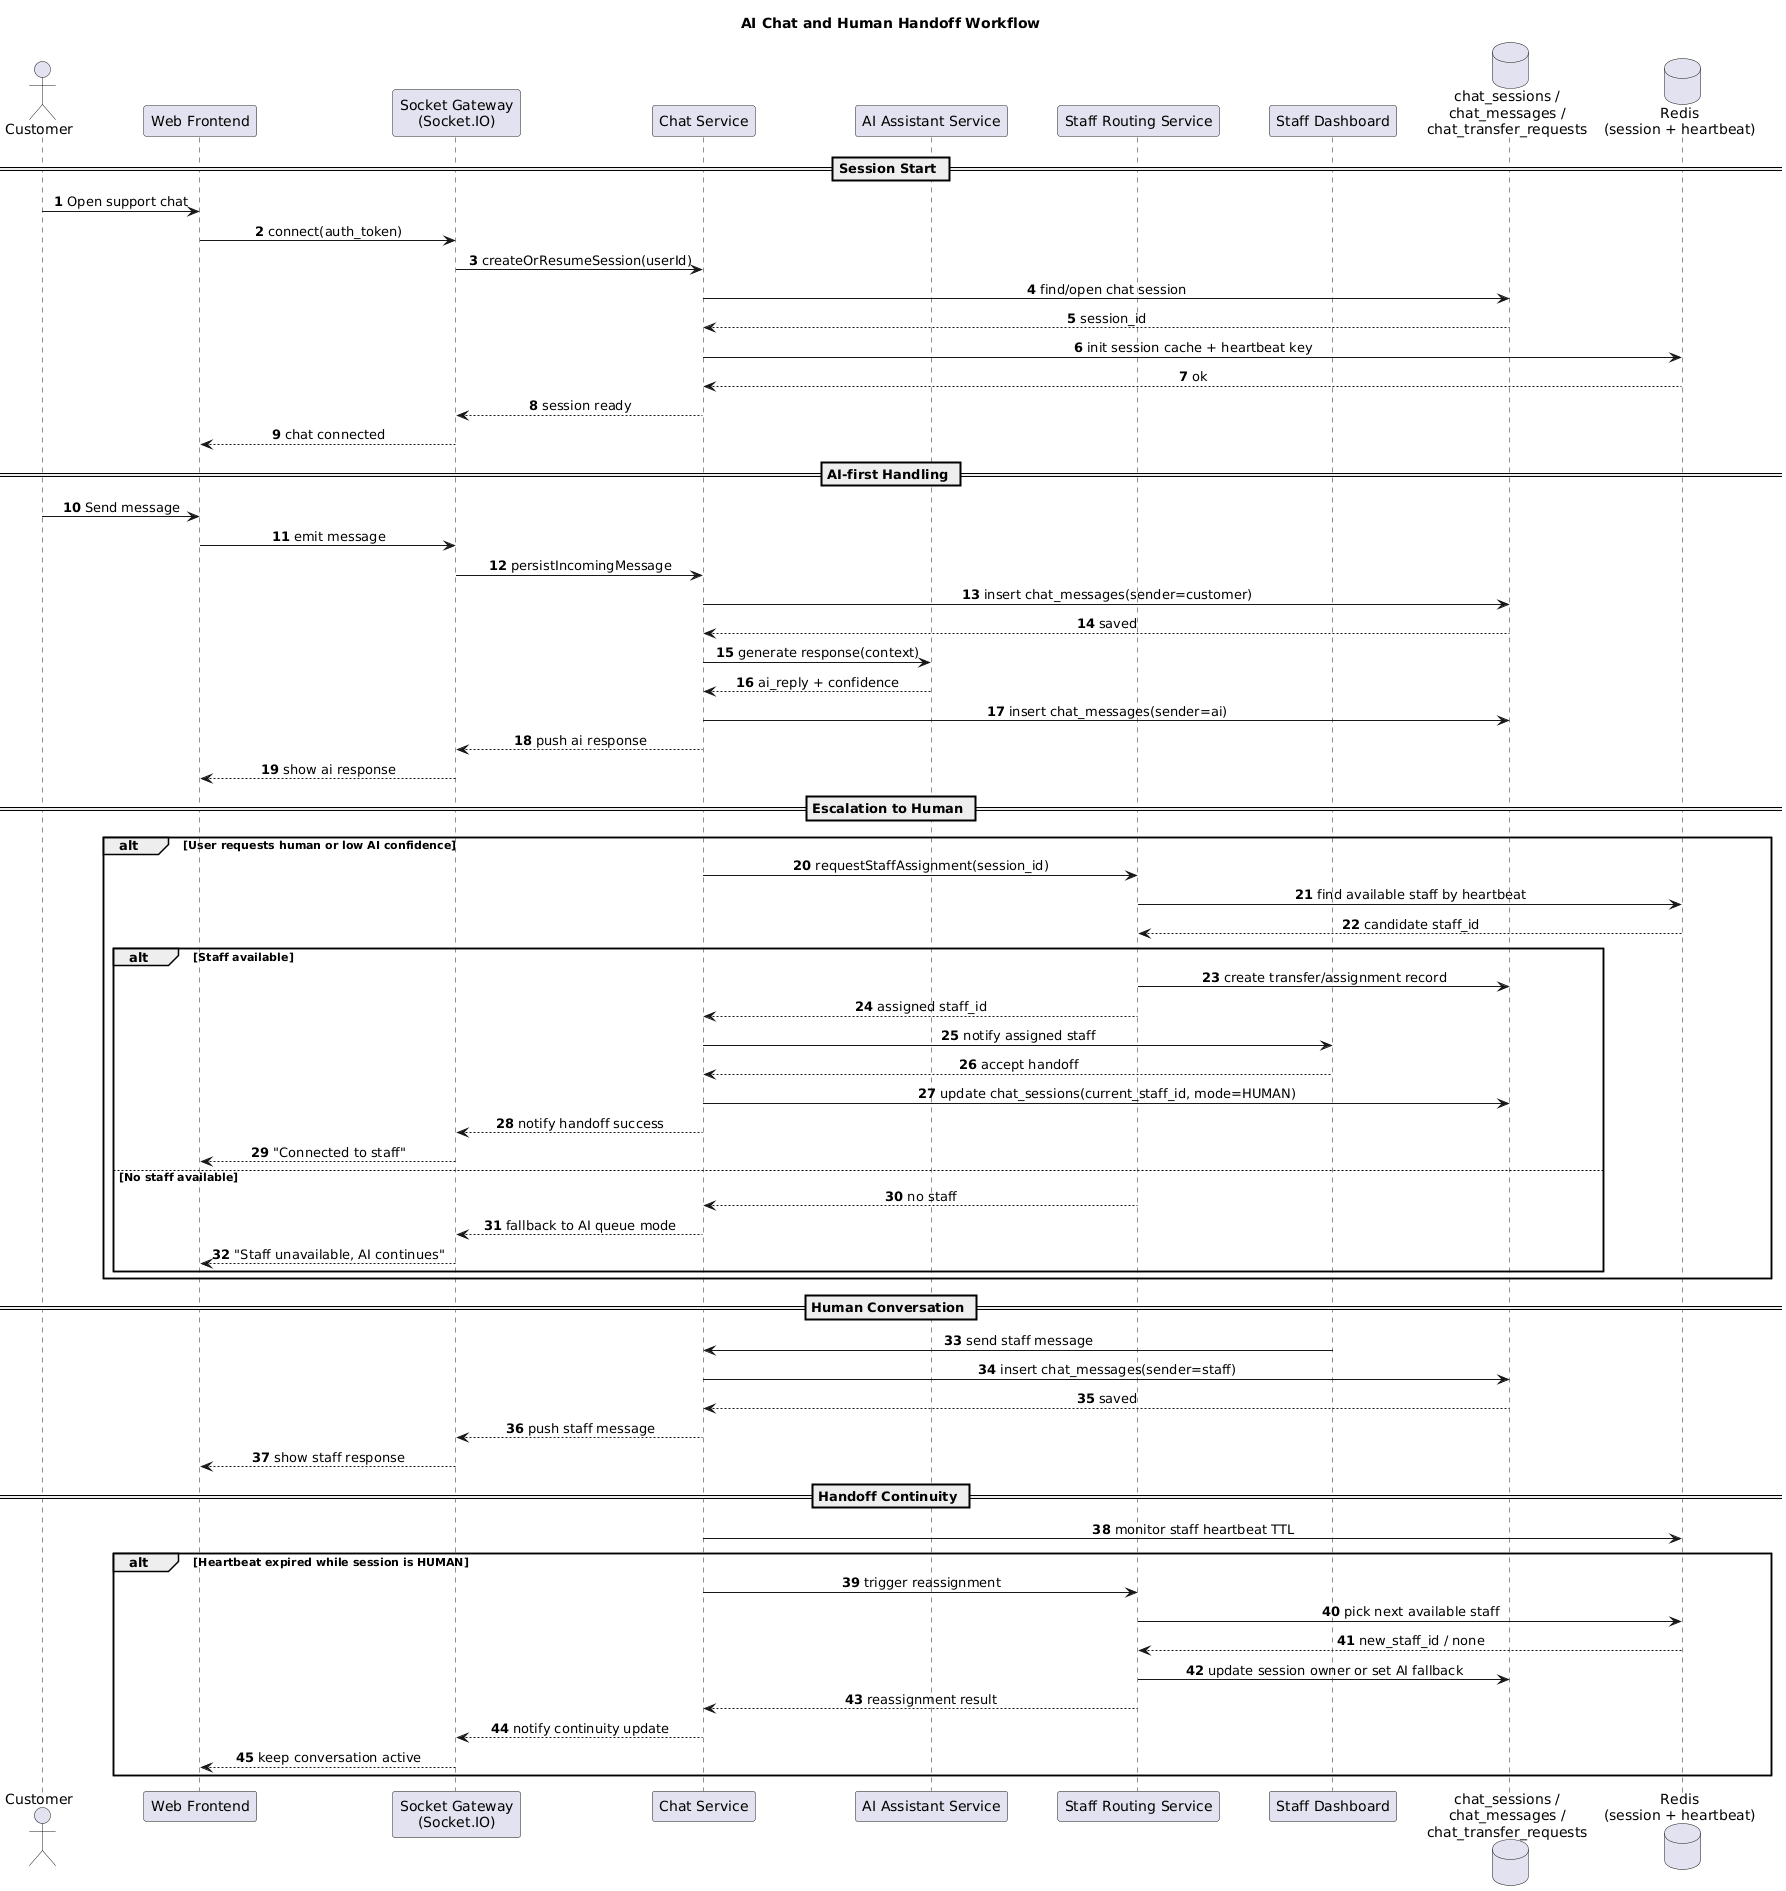
\includegraphics[width=0.9\textwidth]{figures/ch3_chat_handoff_flow.png}
\caption{AI Chat and Human Handoff Workflow}
\label{fig:method-chat-handoff-workflow}
\end{figure}

\subsection{Reservation Expiry and Staff Reassignment Workflow}

Two reliability workflows are modeled in this thesis implementation:
\begin{itemize}
    \item Reservation expiry rollback for stale pending orders.
    \item Staff heartbeat expiry and session reassignment for support continuity.
\end{itemize}

\begin{figure}[H]
\centering
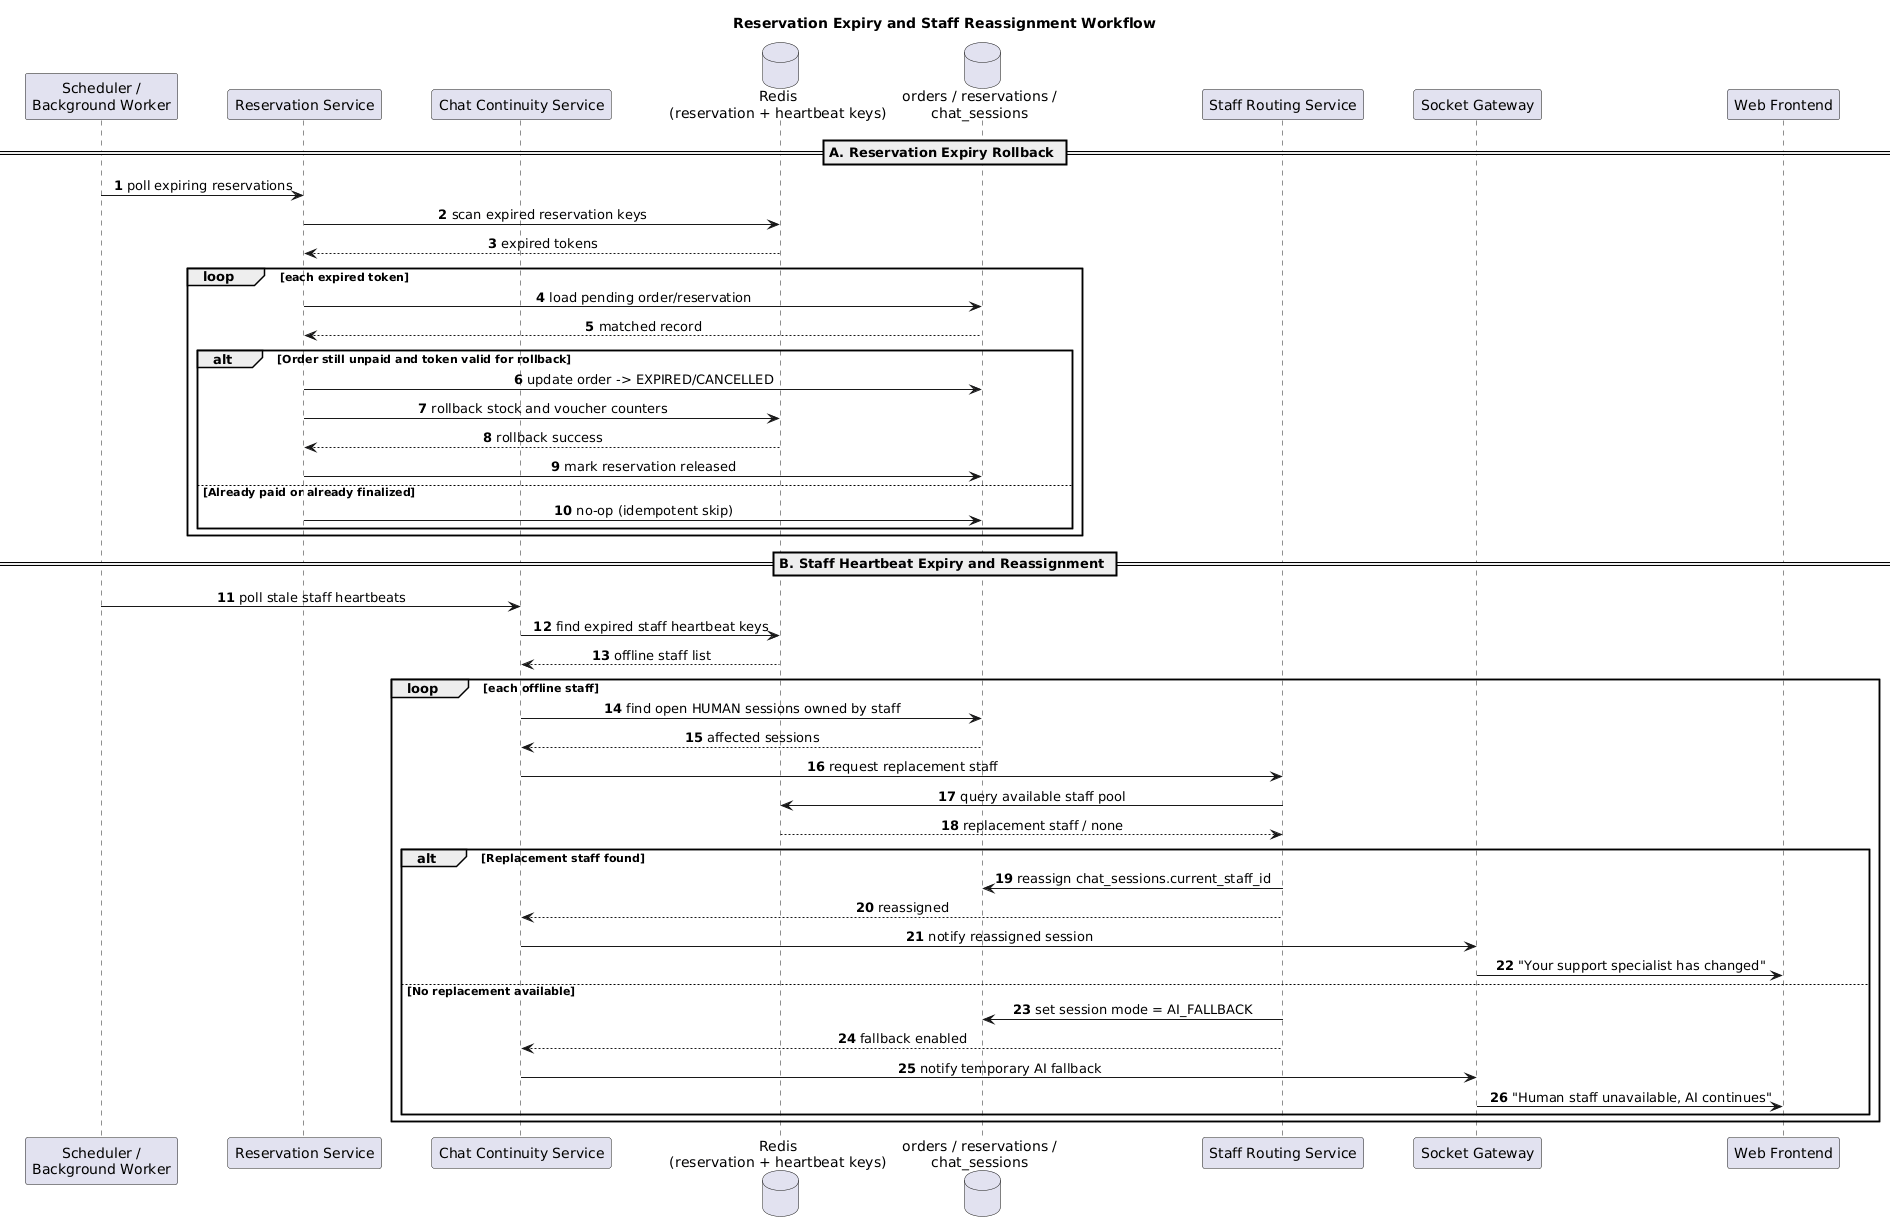
\includegraphics[width=0.9\textwidth]{figures/ch3_reservation_reassignment_flow.png}
\caption{Reservation Expiry and Staff Reassignment Workflow}
\label{fig:method-expiry-reassignment-workflow}
\end{figure}

\section{Evaluation Methodology}

\subsection{Evaluation Scenarios}

The system is evaluated using scenario-based testing:
\begin{itemize}
    \item Standard user purchase flow from login to paid order.
    \item Concurrent checkout on limited stock and discount quotas.
    \item Delayed and repeated payment callback handling.
    \item AI chat escalation and reassignment when staff disconnects.
\end{itemize}

\subsection{Evaluation Metrics}

\begin{table}[H]
\centering
\caption{Evaluation Metrics by Concern}
\label{tab:method-evaluation-metrics}
\begin{tabular}{|p{2.8cm}|p{8.6cm}|}
\hline
\textbf{Concern} & \textbf{Metric Examples} \\
\hline
API performance & p50/p95 latency, throughput, timeout rate \\
\hline
Transactional reliability & reservation rollback success rate, duplicate callback safety \\
\hline
Realtime support & chat response delay, handoff delay, reassignment delay \\
\hline
Security correctness & invalid token rejection, invalid signature rejection \\
\hline
\end{tabular}
\end{table}

\section{Chapter Summary}

This chapter defines the methodology used to design the backend system and to model critical workflows before implementation. The next chapter presents how these designs are realized in the actual backend modules and services.
